\documentclass[a4paper,11pt]{report}

\usepackage[english]{babel}
\usepackage{a4wide}
\usepackage{graphicx}
\usepackage{wasysym}
\usepackage[font=small,labelfont=sf,textfont=sf]{caption}
\usepackage{hyperref}
\usepackage[sf]{titlesec}
\usepackage{lscape}
\usepackage{listings}
\usepackage{fancybox}
\usepackage{mdwlist}
\usepackage{fancyhdr}
\usepackage{xcolor}

\newcommand{\att}[1]{\texttt{#1}}
\newcommand{\meth}[1]{\texttt{#1()}}
\newcommand{\cls}[1]{\textsf{#1}}
\newcommand{\prop}[1]{\texttt{#1}}

\newcommand{\ctx}{\cls{Context}}
\newcommand{\sig}{\cls{Signal}}
\newcommand{\rd}{\cls{Reader}}
\newcommand{\rderr}{\cls{ReadError}}
\newcommand{\wrt}{\cls{Writer}}
\newcommand{\wrterr}{\cls{WriteError}}
\newcommand{\module}[1]{\textsc{#1}}
\newcommand{\graph}{\cls{Graph}}
\newcommand{\fig}{\cls{Figure}}
\newcommand{\cursor}{\cls{Cursor}}
\title{{\sc ioscopy}\\A viewer for plotting electrical simulation results\\User Manual}
\author{Arnaud Gardelein}

\hypersetup{
colorlinks=true,
linkcolor=black,
anchorcolor=black,
citecolor=black,
filecolor=black,
menucolor=black,
pagecolor=black,
urlcolor=black,
}

% From mdwlist
\renewenvironment{description}{%
\begin{basedescript}{%
\renewcommand{\makelabel}[1]{\bfseries##1}%
}%
}{%
\end{basedescript}%
}

\begin{document}
\sf
\maketitle
\begin{abstract}
% data plotter
% post-processing
% result viewer
% primarily targeted for electrical simulation results
% can be extended beyond that
% update and dependency tracking 
% which aims to simplify the development workflow
% interactive

Oscopy is an interactive oscilloscope written in python designed to simplify the electrical design workflow.
It allow to read, view and post-process signals with support for automatic dependency tracking.
File re-reading (updates) can be triggered by external applications like gEDA suite through D-Bus messaging system, and then Oscopy can call netlist generator and electrical simulator programs automatically.
As oscopy is built on top of IPython, post-processing include as well as simple arithmetics operation as complex functions like FFT.
Oscopy can be easily extended to a multi-purpose viewer, as adding new data file formats and new types of plots is really easy.


This document covers the user interface and command description.
% TODO: Update the abstract including short description of ioscopy and GUI
\end{abstract}

\lstset{basicstyle=\ttfamily,backgroundcolor=\color{gray!10},basewidth=0.5em,fontadjust=true}
\pagestyle{fancy}
\lhead{}
\cfoot{}
\rhead{\textsf{\leftmark}}
\rfoot{\textsf\thepage}
\chapter{Introduction}
\label{sec:intro}
% >       * create a central design document that lists all important
% >         concepts/classes (Signal, Figure, ...) and explains interactions
% >         between them; this would really help a lot
% This one is more important. When we figure out and specify how various
% object interact between themselves, we're practically done. Then all the
% code just follows naturally.
In the electrical system design workflow, viewing results from analog simulation or experi\-ment is not a trivial task: there exist numerous different program with even more different file formats, the user interface has to be friendly and functional, and the program should be memory efficient due to the number of data points per file that can quickly grow.

\section{Rationale}
The gEDA suite contains mainly all tools required to design electrical boards, from scheme drawings to PCB routing.
There already exist several programs to view analog simulation results: gwave, GSpiceUI, dataplot.

Gwave is designed as a waveform viewer, and can read text files as well as binary files generated by Spice2, Spice3, ngspice, CAzM or gnucap.
The user interface supports drag and drop signals onto graphs, vertical bar cursors, multiple files and multiple panes.

GSpiceUI is more focused on the interaction between the user and the simulation program: it imports the schematic from gschem, allows the user to build the file to be used by the simulation and plot the results, eventually using GWave.

Dataplot has support for formats like gnucap, ngspice, hdf5 and touchstone.
The user interface has tabs for multiple plots and presents the data in a hierarchical manner.

Another way of viewing results is to use Octave (and generally gnuplot).
This approach enables one to post-process the results with operations such as FFT, diff.
Support for multiple figures is present.
Octave support HDF5 file format and tab-separated text-based files such as gnucap output.
The user interaction is essentially based on the command line interface.

The idea behind Oscopy is to combine the best of these approaches into a single, easily extendable program.
In this purpose, it has features such as multiple plots, multiple windows, different plot types (linear, log) and allows the user to do math with data, including basic operations, trigonometry, fft, diff.
It supports the gnucap file format for input and output, and has an update mechanism to reread data from files.
New file formats and new graph types can be added by following the guidelines presented in this document.

\section{Oscopy and IOscopy: the core and the app}
To enable reuse and make it flexible, Oscopy has two main components:
\begin{description}
\item[Oscopy] the core of it which gather all the framework API about file operations, signals management, figures and graph handling
\item[IOscopy] the application based on top of IPython which provide the command line interface
\end{description}
This means that IOscopy is just an application of using Oscopy core.
As of today the term \textsl{Oscopy} means either Oscopy or IOscopy and when differentiation is needed \textsl{oscopy-core} for the framework and either \textsl{oscopy-ipython} or \textsl{IOscopy} for the IPython application.

The framework API oscopy-core is described in oscopy-api.pdf that is usually installed at the same place of the this manual; typically \texttt{/usr/share/doc/oscopy}.
The present document is only about the application IOscopy.

\section{Supported input data formats}
Reading data files is performed using Oscopy. Supported formats are:
\begin{description}
\item[Gnucap] Text format from Gnucap
\item[Cazm] Text format from CaZM
\item[Nsout] NanoSim format from Synopsis; \textit{Independent variable assumed to be \texttt{Time}}
\item[Spice2raw] Berkeley Spice2G6 raw format; \textit{Only one dataset per file, \texttt{Date} and \texttt{Time} fields not processed}
\item[Spice3raw] Berkeley Spice3 format; \textit{\textbf{ascii} and \textbf{binary} formats supported, real and complex numbers supported. Only one simulation per file.}
\item[Hspice] Hspice format; \textit{\textbf{ascii} and \textbf{binary} formats supported. Only one sweep per file. Auto signals are note returned, only probe signals are. Endianness is not managed in binary mode.}
\item[Touchstone] Touchstone s2p and co. from IBIS Open Forum; \textit{Version 1 and 2.0 supported. for version 1 uses the file extension to determine the number of ports ('.snp' where n is 1-4). Noise parameter data is read and stored in self.info['noise\_param']. Mixed mode parameters of version 2.0 not supported.}
\end{description}

\section{Supported output format}
Writing data files is performed using Oscopy. Supported formats are:
\begin{description}
\item[gnucap] Text format from Gnucap
\end{description}

\section{Supported plots}
Available Graphs are:
\begin{description}
\item[linear] Standard 2D plot with X and Y axis being either linear or logarithmic
\end{description}


\chapter{IOscopy: Oscopy on top of IPython}

%\section{Purpose}
% TODO: Why using ipython: CLI already there, oscopy as a python module, power of ipython behind, flexibility
\section{First steps}
\subsection{Install dependencies}
Requested dependencies for building and downloading:
\begin{itemize}
\item    autoconf
\item    gettext
\item    intltool $\ge$ 0.41.0
\item    git
\end{itemize}

\noindent Requested dependencies for execution:
\begin{itemize}
\item    python
\item    python--gtk
\item    ipython $\ge$ 0.13
\item    python--numpy
\item    python--matplotlib
\item    python--dbus
\item    python--xdg
\end{itemize}

\noindent Optional dependencies to run demo/demo.oscopy
\begin{itemize}
\item    geda--gaf and more specifically gschem and gnetlist
\item    gnucap
\end{itemize}

\subsubsection{Debian}
Tested on stable (squeeze) and unstable (sid). Will not install on stable due to default release ipython 0.10.

Install git, autotools and related packages:
\begin{lstlisting}
# apt-get git autoconf gettext intltool python-gtk2-dev
\end{lstlisting}
Install oscopy dependencies:
\begin{lstlisting}
# apt-get install ipython python-matplotlib
\end{lstlisting}
Optional: to execute demo.oscopy script install geda and gnucap:
\begin{lstlisting}
# apt-get install geda gnucap
\end{lstlisting}

\subsubsection{Ubuntu}
Tested on Ubuntu 12.10 Quantal Quetzal.

Install git, autotools and related packages:
\begin{lstlisting}
$ sudo apt-get install git autoconf gettext intltool python-gtk2-dev
\end{lstlisting} %$
Install oscopy dependencies:
\begin{lstlisting}
$ sudo apt-get install ipython python-matplotlib
\end{lstlisting} %$
Optional: to execute demo.oscopy script install geda and gnucap:
\begin{lstlisting}
$ sudo apt-get install ipython python-matplotlib
\end{lstlisting} % $

\subsubsection{Fedora}
Tested on Fedora 18.

Install git, autotools and related packages (maybe needed to run the command twice ?):
\begin{lstlisting}
# yum install git autoconf gettext intltool pygtk2-devel gcc
\end{lstlisting}
Install oscopy dependencies:
\begin{lstlisting}
# yum install ipython dbus-python 
\end{lstlisting}
Optional: to execute demo.oscopy script install geda and gnucap:
\begin{lstlisting}
# yum install geda-gaf gnucap 
\end{lstlisting}
Note that in Fedora 18 default geda-gaf and gnucap appear to be very old version and might not run demo/demo.oscopy correctly. 

\subsection{Download the source}
The source can be downloaded from repo.or.cz: \href{http://repo.or.cz/w/oscopy.git}{http://repo.or.cz/w/oscopy.git}

To download it:
\begin{lstlisting}
$ git clone git://repo.or.cz/oscopy.git
\end{lstlisting} % $

Optional: to use the experimental branch:
\begin{lstlisting}
$ cd oscopy
$ git pull git://repo.or.cz/oscopy.git experimental
\end{lstlisting}

\subsection{Install oscopy}
IOscopy shall be compiled and installed on the system:
\begin{lstlisting}
$ cd oscopy
$ ./autogen.sh && ./configure && make install
\end{lstlisting}
Once installed, \texttt{PYTHONPATH} might need some update, for example if you install it in \texttt{\$\{HOME\}/geda}, to launch oscopy you might need the following line:
\begin{lstlisting}
$ export PYTHONPATH=${HOME}/geda/lib/python2.X/site-packages:$PYTHONPATH
$ export PATH=$PATH:${HOME}/geda/bin
\end{lstlisting}
To use gschem integration, you will need to use the same \texttt{--prefix} that you used to install gschem. 

\subsection{Getting Started}
To run the program, just do 
\begin{lstlisting}
ioscopy
\end{lstlisting}
This assume that ioscopy is in your \texttt{PATH}.

A sample circuit is provided for demonstration purposes. 
\begin{lstlisting}
$ cd demo
$ ioscopy
\end{lstlisting}
Just select ``File$>$Run Netlister and simulate...'' and fill in the window with the commands provided below: 
\begin{itemize}
\item For netlister: \lstinline!gnetlist -g spice-sdb -s -o demo.net demo.sch!
\item For simulator: \lstinline!gnucap -b demo.net!
\end{itemize}
then in the terminal window:
\begin{lstlisting}
oscopy> oexec demo.oscopy
\end{lstlisting}

\subsection{Integration with gschem}
\label{sec:gschemint}
To use gschem integration, add the following line to your gschemrc:
\begin{lstlisting}
(load-from-path "oscopy.scm")
\end{lstlisting}
On the next start of gschem, you should see the oscopy menu. Note that you should have done \texttt{./configure --prefix=''same prefix as gschem''} Then assuming you are in the oscopy directory: 
\begin{itemize}
\item     launch gschem
\item    open demo/demo.sch
\item    oscopy$> >$Launch oscopy
\item    \lstinline!oscopy> oexec demo.oscopy!
\item    Once the script finished to execute, go back to gschem and change the value of a component e.g. the capacitor C.
\item    oscopy$> >$Update oscopy
\item    once netlister and simulator ran, figures should have changed, e.g. figure 3 \texttt{vout} should have moved and \texttt{vo} not.
\end{itemize}

\section{IOscopy interfaces}
IOscopy has three main interfaces:
\begin{description}
\item[The command line] which is used to enter commands
\item[The Main Window] includes general file I/O, windows list and signal tree
\item[The figures] when instantiated
\end{description}
The two former are specific to IOscopy while the latter is a specialisation of Oscopy Figure.
The command line is an IPython application with customisation for Signal management.
All IOscopy commands are implemented as magic functions.

The Main Window and the figures form the IOscopy GUI and are implemented using GTK libraries.

\section{Command line options}
Command line options are reported in Tab.~\ref{tab:clio}.
\begin{table}[htbp]
  \centering\sf
  \begin{tabular}{ll}
    \hline
   -b&	Execute an oscopy command file\\
   -h&	Show this help message\\
   -i&	Resume to command line executing after batch file\\
   -q&	Disable banner printing\\
   \hline
  \end{tabular}
  \caption{Command line options}
  \label{tab:clio}
\end{table}
\section{IOscopy Commands Reference}
% TODO: Detailled description of ioscopy commands with an example for each one, assuming the demo/demo.oscopy script conditions
This section describes the IOscopy commands. Unless otherwise noticed, examples assume that \texttt{demo/demo.oscopy} has been run.

\newcommand{\ocmd}[2]{\vspace{3eX}\noindent\fbox{\begin{minipage}{\linewidth}\large\noindent\textbf{#1} #2\end{minipage}}\vspace{1eX}}

\ocmd{oadd}{SIG [, SIG [, SIG]...]}
   Add a graph to the current figure. Figure and graph are instanciated if not present.

\begin{lstlisting}
   oscopy> oselect 1-1
   oscopy> oadd vgs
\end{lstlisting}

\ocmd{ocreate}{[SIG [, SIG [, SIG]...]]}
   Create a new figure, set it as current, add the signals in a first graph.

\begin{lstlisting}
   oscopy> ocreate vgs,vds
\end{lstlisting}

\ocmd{ocontext}{\ }
   Return the Context object used within ioscopy.
 Use it only if you want to have direct access to internal ioscopy objects.

\ocmd{odelete}{GRAPH\#}
   Delete a graph from the current figure.

\begin{lstlisting}
   oscopy> odelete 1
\end{lstlisting}

\ocmd{odestroy}{FIG\#}
   Destroy a figure

\begin{lstlisting}
   oscopy> odestroy 3
\end{lstlisting}

\ocmd{oexec}{FILENAME}
   Execute commands from file.

   This following example assumes that demo/demo.oscopy has \textbf{not} been run.

\begin{lstlisting}
   oscopy> oexec demo/demo.oscopy
\end{lstlisting}

\ocmd{ofactors}{X, Y}
   Set the scaling factor of the graph (in powers of ten). Use \texttt{auto} for automatic scaling factor.

\noindent   The following example sets the scale factor at 1e-3 for X axis and 10e6 for Y axis
\begin{lstlisting}
   oscopy> oselect 1-1
   oscopy> ofactor -3, 3
\end{lstlisting}

\ocmd{ofiglist}{\ }
   Print the list of figures. The layout of the figure is indicated, and the graph mode as well as the Signals are shown. The current figure and graph are marked with a star.
\begin{lstlisting}
   oscopy>ofiglist
     Figure 1: horiz
      Graph 1 : (linear) vgs
      Graph 2 : (linear) vsqu
     Figure 2: quad
      Graph 1 : (linear) iRD
      Graph 2 : (linear) vgs
      Graph 3 : (linear) vds vgs
      Graph 4 : (linear) vds
     Figure 3: horiz
      Graph 1 : (linear) vout vo
     Figure 4: horiz
      Graph 1 : (linear) vsqu
      Graph 2 : (linear) vsqufft
      Graph 3 : (linear) v1
   * Figure 5: horiz
       * Graph 1 : (linear) vs
\end{lstlisting}

\ocmd{ofreeze}{SIG [, SIG [, SIG]...]}
   Do not consider signal for subsequent updates. See also \textbf{ounfreeze}.
\begin{lstlisting}
   oscopy> ofreeze vout,vds
\end{lstlisting}

\ocmd{ogui}{\ }
   Show the GUI window if it was closed.

\ocmd{oimport}{SIG [, SIG [, SIG]...]}
   Import a list of signals into oscopy to handle dependencies during updates
\begin{lstlisting}
   oscopy> pwr=iRD*vds
   oscopy> oimport pwr
   oscopy> ocreate pwr
   oscopy> oupdate  #if iRD or vds changed, pwr will be automatically updated
\end{lstlisting}

\ocmd{oinsert}{SIG [, SIG [, SIG]...]}
   Insert a list of signals into the current graph
\begin{lstlisting}
   oscopy> oselect 1-1
   oscopy> oinsert vds
\end{lstlisting}

\ocmd{olayout}{horiz$|$vert$|$quad}
   Define the layout of the current figure
   \begin{description}
   \item[olayout horiz] Graphs are stacked from top to bottom
   \item[olayout vert] Graphs are side by side from left to right
   \item[olayout quad] One graph per figure corner
   \end{description}
\begin{lstlisting}
   oscopy> oselect 2-1
   oscopy> olayout horiz
   oscopy> olayout vert
   oscopy> olayout quad
\end{lstlisting}

\ocmd{omode}{MODE}
   Set the type of the current graph of the current figure\\
   Available modes:
   \begin{description}
   \item[omode lin]      Linear graph
   \end{description}

\ocmd{orange}{[x$|$y min max]$|$[xmin xmax ymin ymax]$|$[reset]}
   Set the axis range of the current graph of the current figure
   \begin{description}
   \item[orange x xmin xmax] set x axis range
   \item[orange y ymin ymax] set y axis range
   \item[orange xmin xmax ymin ymax] set both axis range
%   \item[orange reset] set automatic range on both axis
   \end{description}
\begin{lstlisting}
   oscopy> oselect 1-1
   oscopy> orange x 0 1
   oscopy> orange y -4 12
   oscopy> orange 0.5 0.6 -2 2
\end{lstlisting}

\ocmd{oread}{DATAFILE}
   Read signal file
\begin{lstlisting}
   oscopy> oread demo/tran.dat
\end{lstlisting}

\ocmd{orefresh}{FIG\#$|$current$|$all$|$on$|$off}
   Force/toggle autorefresh of current/\#/all figures on update
   \begin{description}
   \item[orefresh FIG\#] refresh figure \#
   \item[orefresh current] refresh current figure
   \item[orefresh all]  refresh all figures
   \item[orefresh on] turn on autorefresh on Signal updates
   \item[orefresh off] turn off autorefresh on Signal updates
   \end{description}

\begin{lstlisting}
   oscopy> orefresh 3
   oscopy> orefresh on
\end{lstlisting}

\ocmd{oremove}{SIG [, SIG [, SIG]...]}
   Delete a list of signals into from current graph
\begin{lstlisting}
   oscopy> oselect oselect 2-3
   oscopy> oremove vds
\end{lstlisting}

\ocmd{oscale}{[lin$|$logx$|$logy$|$loglog]}
   Set the axis scale
   \begin{description}
   \item[oscale lin] Set linear scale on both axis
   \item[oscale logx] Set log scale on x axis and linear scale on y axis
   \item[oscale logy] Set linear scale on x axis and log scale on y axis
   \item[oscale loglog] Set log scale on both axis
   \end{description}

\begin{lstlisting}
   oscopy> oselect 3-1
   oscopy> oscale logx
   oscopy> oscale loglog
\end{lstlisting}

\ocmd{oselect}{FIG\#-GRAPH\#}
   Select the current figure and the current graph
\begin{lstlisting}
   oscopy> oselect 2-1
\end{lstlisting}

\ocmd{osiglist}{\ }
   List loaded signals
\begin{lstlisting}
   oscopy> siglist
   Name	Unit	Ref	Reader	Last updated (sec)
   vds	V	Time	demo/irf540.dat	128
   iRD	A	Time	demo/irf540.dat	128
   vgs	V	Time	demo/irf540.dat	128
   vsqu	V	Time	demo/tran.dat	124
   v1	None	Time	v1=((vsqu * 3) + 10)	123
   vout	V	Freq	demo/ac.dat	126
   vs	None	Time	vs=sin((Time * 1000000.0))	121
   vs2	V	Time	vs2=sin((Time * 1000000.0))	121
   vo	V	Freq	vo=vout	121
   vsqufft		Frequency	vsqufft=fft(vsqu)	124
\end{lstlisting}

\ocmd{ounfreeze}{SIG [, SIG [, SIG]...]}
   Consider signal for subsequent updates. See also \textbf{ofreeze}
\begin{lstlisting}
   oscopy> ounfreeze vout,vds
\end{lstlisting}

\ocmd{ounit}{[XUNIT,] YUNIT}
   Set the unit to be displayed on graph axis
   \begin{description}
   \item[ounit XUNIT, YUNIT] Set both axis unit
   \item[ounit YUNIT] Set Y axis unit
   \end{description}

\begin{lstlisting}
   oscopy> oselect 3-1
   oscopy> ounit W      # Set Y axis unit
   oscopy> ounit /s,W   # Set both axis unit
   oscopy> ounit Hz, V
\end{lstlisting}

\ocmd{oupdate}{\ }
   Reread data files.

\begin{lstlisting}
   oscopy> oupdate
\end{lstlisting}

\ocmd{owrite}{format [(OPTIONS)] FILE SIG [, SIG [, SIG]...]}
   Write signals to file.
Options common to all formats are:
\begin{description}
\item[ow] If \texttt{True} or 1 overwrite existing file
\end{description}

\noindent This example writes signals v1 and vsqu to the file \texttt{demo/res.dat} using format gnucap format,
   overwriting the file if it already exists.
\begin{lstlisting}
   oscopy> owrite gnucap (ow:1) demo/res.dat v1,vsqu
\end{lstlisting}
\newpage
\chapter{Oscopy GUI}
% TODO: Description of the GUI interface, main window, menus, contextual menus, buttons
The Graphical User Interface of oscopy is composed of several windows (Figure \ref{fig:screenshot}):
\begin{itemize}
\item The command line terminal
\item The main window
\item The (many) figures windows
\end{itemize}
The next paragraphs describe the two last types.

\begin{figure}[htbp]
  \centering
  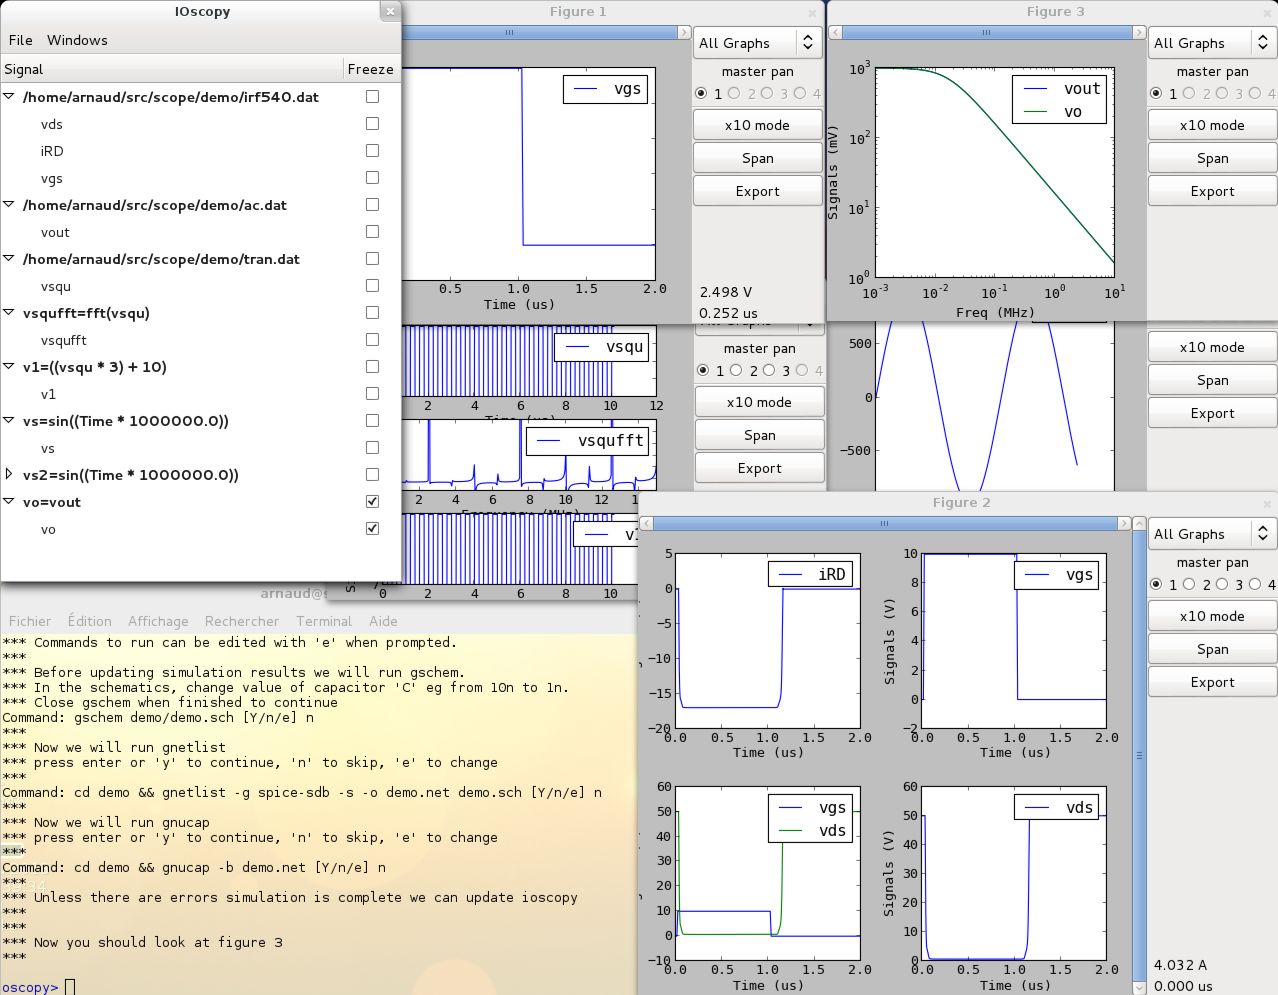
\includegraphics[width=.8\textwidth]{../png/ioscopy.png}
  \caption{ioscopy after running \texttt{demo/demo.oscopy}}
  \label{fig:screenshot}
\end{figure}

\section{The main window}
This is the first window that you will see when starting ioscopy.
At anytime, it can be shown again by calling the command \texttt{ogui} from the terminal if closed.

It contains the list of Readers and their Signals currently handled by ioscopy.
Double--clicking on a Signal inserts it in a new Figure.

Each Signal 'freeze' status can be toggled using the checkbox located in the right column.
Toggling the checkbox for a Reader set the status for all the signals contained in the Reader.

The 'File' menu:
\begin{description}
\item[Add file(s)...] To read Signals from file(s)
\item[Update] To read Signals from file(s) again
\item[Execute script...] To read ioscopy commands from file
\item[New Math Signal] To compute a new Signal from existing ones
\item[Run netlister and simulate] To generate the netlist, run the simulator and eventually update the Signals (Figure~\ref{fig:netnsim})
\item[Quit] Exit ioscopy
\end{description}

\noindent The 'Windows' menu contains the list of the windows, and select one to show it.

% description des menus
% description de la liste (+ freeze fichier entier ou signal par signal)

\begin{figure}[htbp]
  \centering
  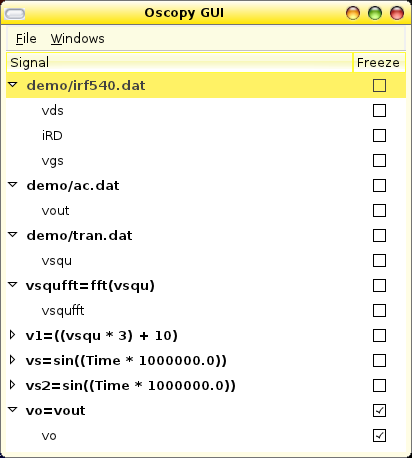
\includegraphics[scale=.5]{../png/ioscopy-gui.png}
  \caption{The main window}
  \label{fig:mainwin}
  \begin{minipage}{.45\linewidth}
    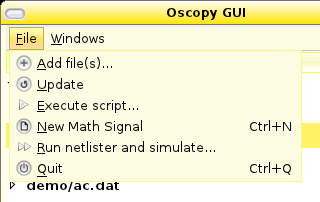
\includegraphics[scale=.5]{../png/ioscopy-file.png}
    \caption{The 'File' menu}
    \label{fig:filemenu}
  \end{minipage}
  \begin{minipage}{.45\linewidth}
    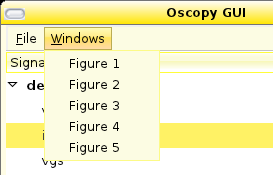
\includegraphics[scale=.5]{../png/ioscopy-window.png}
    \caption{The 'Window' menu}
    \label{fig:windowmenu}    
  \end{minipage}

  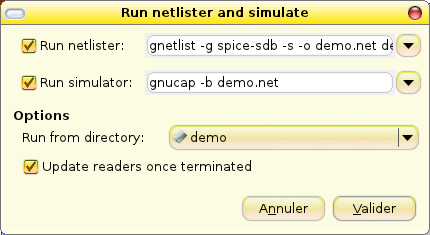
\includegraphics[scale=.5]{../png/ioscopy-netnsim.png}
  \caption{The 'Run netlister and simulate' window. Call third party programs to generate oscopy input files. Can be toggled with the checkboxes. Setting are saved in .config/oscopy/gui file}
  \label{fig:netnsim}

\end{figure}

\noindent Available mouse operations:
\begin{description}
\item[left] Select signal
\item[double left] Insert signal in new Figure
\item[right] Show 'Insert signal' menu
\end{description}

\section{The Figure windows}

% description de l'agencement de la fenêtre
% description du menu contextuel et des sous-menus
Each Figure window is composed of two parts:
\begin{itemize}
\item On the top part, a zone containing up to 4 graphs
\item On the bottom part, the Matplotlib toolbar
\item On the right part, the Operation bar
\end{itemize}
A contextual menu is available for each graph, raised by a right-click on the mouse button.
Access to most of the ioscopy functionality is possible through this menu:
\begin{itemize}
\item Add/delete graph
\item Layout (Figure~\ref{fig:layout})
\item Range settings (Figure~\ref{fig:range})
\item Unit settings (Figure~\ref{fig:units})
\item Scale (Figure~\ref{fig:scale})
% Insert Signal not available anymore as per commit 084a6d87:
% the call to Context.create is delegated to UI. Furthermore, the Graph is
% not anymore aware of Context's Signals.
%\item Insert Signal (Figure~\ref{fig:insert})
\item Remove Signal (Figure~\ref{fig:remove})
\end{itemize}

For each Graph, cursors are available through keys (Figure~\ref{fig:cursors}):
\begin{itemize}
\item \texttt{'1'} for first vertical cursor
\item \texttt{'2'} for second vertical cursor
\item \texttt{'3'} for first horizontal cursor
\item \texttt{'4'} for second horizontal cursor
\end{itemize}
The value of each cursor is displayed on the bottom part of the graph, and the difference when both cursors are activated.

\noindent Available mouse operations:
\begin{description}
\item[left] In a graph and when 'span' is selected, define region for zooming
\item[roll] In a graph, Zoom in / Zoom out
%\item[double left] Insert signal in new Figure
\item[right] Show 'Contextual signal' menu. Sensitive to position, e.g. Graph-related items are only available when mouse is over a Graph.
\end{description}


\subsection{The Operation Bar}

This bar is used to set options for all the Graphs at the same time or for a particular Graph.
The target Graph is selected through the top-most combo-box.
\begin{description}
\item[Master pan] When scroll bars are moved, move also all Graphs with same X unit than selected.
\item[Zoom x10] When enabled, the graph range is expanded at a x10 scale, keeping the center of the view. When disabled, return to full range. E.g. if the initial range is [6 .. 11] and the data range is [0 .. 20], the x10 range will be [7.5 .. 9.5] and will be [0 .. 20] on disabling.
\item[Span] When enabled, use mouse--left to zoom in a region of a Graph (Figure~\ref{fig:span}). Region selection is made upon the Figure layout configuration:
  \begin{description}
  \item[horizontal] Region is selected on X axis
  \item[vertical] Region is selected on Y axis
  \item[quad] Region is selected on both axis
  \end{description}
\item[Export] Save figure as image
\end{description}

\begin{figure}[htbp]
  \centering
  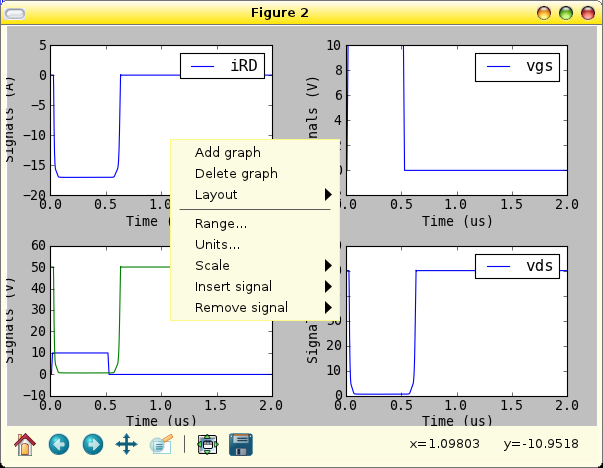
\includegraphics[scale=.5]{../png/ioscopy-figure}
  \caption{A Figure window with the contextual menu.}
  \label{fig:fig}

  \begin{minipage}{0.45\linewidth}
    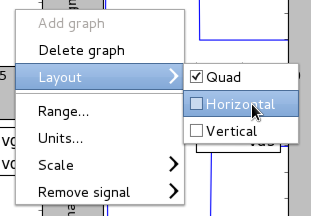
\includegraphics[scale=.5]{../png/ioscopy-layout.png}
    \caption{Layout configuration menu}
    \label{fig:layout}
  \end{minipage}
  \begin{minipage}{0.45\linewidth}
    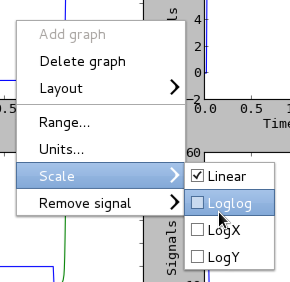
\includegraphics[scale=.5]{../png/ioscopy-scale.png}
    \caption{Scale configuration menu}
    \label{fig:scale}
  \end{minipage}

  \begin{minipage}{0.95\linewidth}
    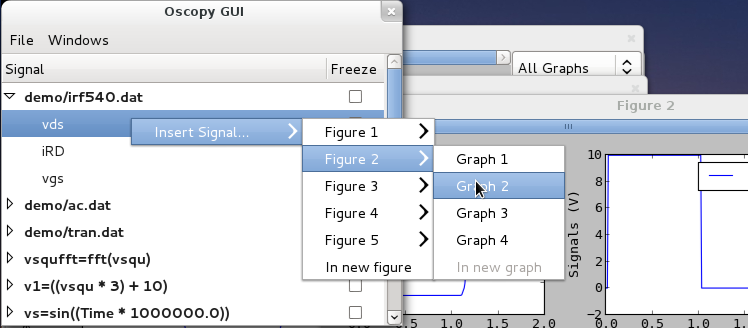
\includegraphics[scale=.5]{../png/ioscopy-insert.png}
    \caption{Insert signal menu}
    \label{fig:insert}
  \end{minipage}

\end{figure}

\begin{figure}[htbp]
  \centering
  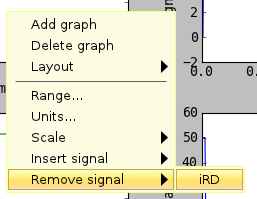
\includegraphics[scale=.5]{../png/ioscopy-remove.png}
  \caption{Remove signal menu}
  \label{fig:remove}

  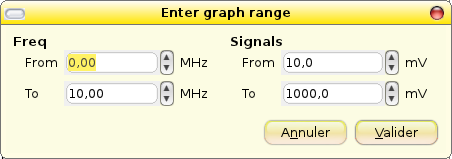
\includegraphics[scale=.5]{../png/ioscopy-range.png}
  \caption{Dialogue to set graph range}
  \label{fig:range}

  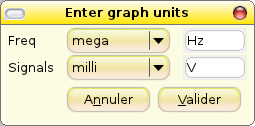
\includegraphics[scale=.5]{../png/ioscopy-units.png}
  \caption{Dialogue to set graph units}
  \label{fig:units}

  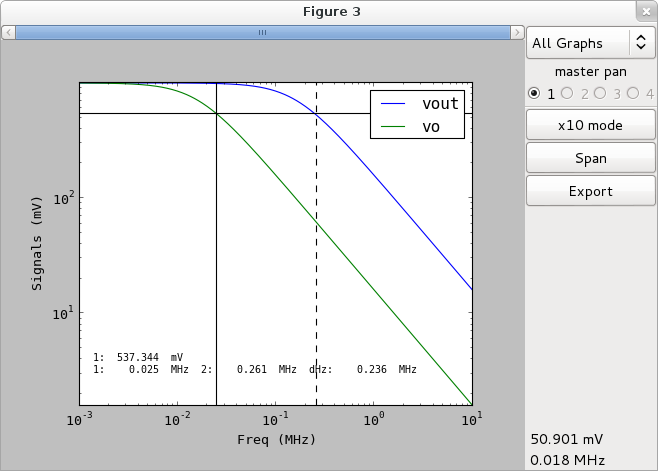
\includegraphics[scale=.5]{../png/ioscopy-cursors.png}
  \caption{Figure with cursors set (after changing capacitance value of \texttt{demo.sch} and running netlister and simulator}
  \label{fig:cursors}

\end{figure}

\begin{figure}[htbp]
  \centering
  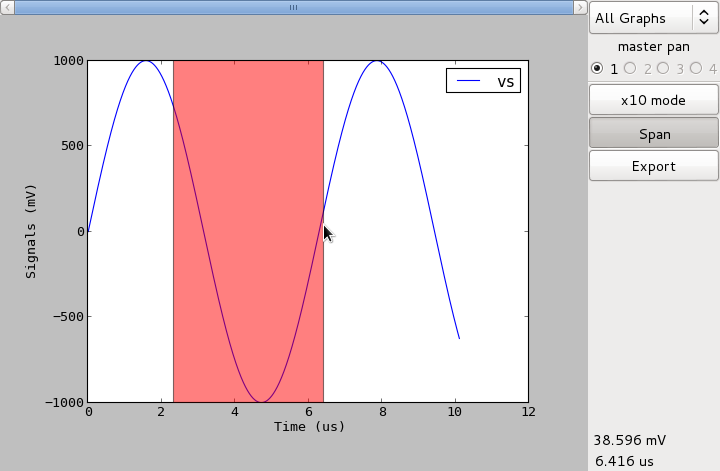
\includegraphics[scale=.5]{../png/ioscopy-span.png}
  \caption{Select region for zooming. Here with horizontal layout.}
  \label{fig:span}
\end{figure}

\appendix
\chapter{IOscopy commands quick reference guide}
\begin{landscape}
  \begin{table}[htbp]
    \centering\sf
    \begin{tabular}{lll}
      \hline
      Command & Arguments & Description \\
      \hline
      oadd & SIG [, SIG [, SIG]...] &Add a graph to the current figure\\
      ocontext& & Return the Context object used within ioscopy.\\
      & &Use it only if you want to have direct access to internal ioscopy objects.\\
      ocreate & [SIG [, SIG [, SIG]...] ]&Create a new figure, set it as current, add the signals\\
      odelete & GRAPH\# &Delete a graph from the current figure\\
      odestroy & FIG\# &Destroy a figure\\
      oexec & FILENAME &execute commands from file\\
      ofactors & X, Y &set the scaling factor of the graph (in power of ten)   use 'auto' for automatic\\
      & & scaling factor e.g. factor -3, 6 set the scale factor at 1e-3 and 10e6\\
      ofiglist & &Print the list of figures\\
      ofreeze & SIG [, SIG [, SIG]...] &Do not consider signal for subsequent updates\\
      ogui & & Show the GUI\\
      oimport& SIG [, SIG [, SIG]...] & Import a list of signals into oscopy to handle dependencies during updates\\
      oinsert & SIG [, SIG [, SIG]...] &Insert a list of signals into the current graph\\
      olayout & horiz | vert | quad&Define the layout of the current figure\\
      omode & MODE &Set the type of the current graph of the current figure\\
      & &Available modes :\\
      & & lin      Linear graph\\
      orange & [x | y min max] | [xmin xmax ymin ymax] &Set the axis range of the current graph of the current figure\\
      oread & DATAFILE &read signal file\\
      orefresh &  FIG\# | on | off | current | all& Force/toggle autorefresh of current/\#/all figures on update\\
      oremove & SIG [, SIG [, SIG]...] &Delete a list of signals into from current graph\\
      oscale & [lin | logx | logy | loglog] &Set the axis scale\\
      oselect & FIG\#-GRAPH\# &Select the current figure and the current graph\\
      osiglist & &List loaded signals\\
      ounfreeze & SIG [, SIG [, SIG]...] &Consider signal for subsequent updates\\
      ounit & [XUNIT,] YUNIT &Set the unit to be displayed on graph axis\\
      oupdate & &Reread data files\\
      owrite & format [(OPTIONS)] FILE SIG [, SIG [, SIG]...] &Write signals to file\\
      \hline
    \end{tabular}
    \caption{Summary of IOscopy commands}
    \label{tab:cmds:summary}
  \end{table}
\end{landscape}


\end{document}

%%% Local Variables:
%%% Local IspellDict: british
%%% mode: latex
%%% TeX-master: t
%%% End:
